\section{Durchführung}

\subsection{Aufbau}

\begin{figure}[h]
    \centering
    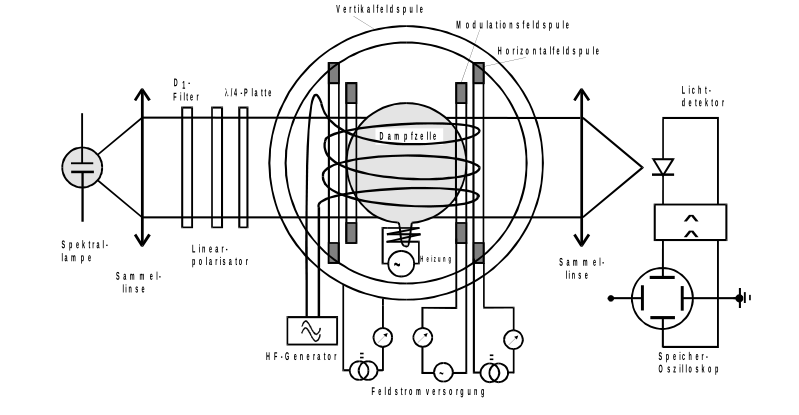
\includegraphics[width=0.7\textwidth]{latex/images/aufbau.PNG}
    \caption{Der Aufbau für das optische Pumpen schematisch dargestellt \protect \cite{V21}.}
    \label{img:aufb}
\end{figure}

\noindent
Der Aufbau des Versuchs ist in Abbildung \ref{img:aufb} schematisch dargestellt.\\
Er teilt sich dabei in einen optischen und einen Messaufbau auf. Der reale optische Aufbau ist in Abbildung
\ref{img:aufb_opt} zu finden und der Messaufbau in Abbildung \ref{img:aufb_mess}.\\
Im optischen Aufbau strahlt eine Rubidium-Spektrallampe auf eine Kollimations-Linse, die den Strahl bündelt.
Anschließend trifft das Licht auf einen Filter, der alle Frequenzen bis auf die $D_1$-Linie von Rubidium, 
mit $\lambda = \SI{794.8}{\nano\metre}$, herausfiltert. Danach wird das Licht erst linear polarisiert um dann mit einer $\frac{\lambda}{4}$-Platte zirkular polarisiert.\\
Dieses Licht trifft dann auf die Dampfzelle, welche den Rubidium-Dampf enthält. 
Der Dampf wird mit einem kleinen Ofen erwärmt, um den optimalen Dampfdruck zu gewährleisten.
Dies sollte eine halbe Stunde vor den Messungen geschehen.\\\\
Die Dampfzelle ist von drei Helmholtzspulen und einer weiteren Spule umgeben.\\
Eine der Helmholtzspulen ist dabei so aufgebaut, dass die Magnetfeldlinien ihres Feldes senkrecht auf dem Tisch stehen.
Dies dient später dazu die vertikale Komponente des Erdmagnetfeldes ausgleichen zu können.\\
Die anderen beiden Helmholtzspulen sind so aufgebaut, dass ihr Feld parallel zum Strahlengang ist.
Eine der Spulen ist die sogenannte Sweep-Spule. 
Für sie kann ein Startwert, ein Endwert und ein Durchlaufzeitraum eingestellt werden, der von dem Feld durchlaufen wirds.\\
Die andere ist die Horizontalfeld-Spule. 
Mit ihr wird ein zusätzliches Feld angelegt, welches auf das Feld der Sweep-Spule addiert wird, da diese nur einen kleinen Feldstärkenbereich abdecken kann.\\
Die letzte Spule ist die RF-Spule oder \enquote*{radio-frequency}-Spule. 
Sie erzeugt ein Magnetwechselfeld, welches die Dampfzelle durchsetzt.\\
Ihre Frequenz kann variiert werden.\\\\ 
Hinter der Dampfzelle im Strahlengang befindet sich noch eine Sammellinse, welche den Lichtstrahl auf einen Photodetektor bündelt.
Dieser ist an ein Oszilloskop und ein Galvanometer angeschlossen.\\
Zusätzlich werden noch Steuergeräte genutzt, mit denen die Stromstärke der Spulen eingestellt werden kann.
Die RF-Spule ist an einen Impulsgenerator angeschlossen, mit dem die Frequenzen varriert werden können.\\


\subsection{Durchführung}

Zuerst werden alle optische Bauteile so im Strahlengang positioniert, dass die am Galvanometer gemessene Stromstärke maximal wird.\\
Anschließend wird bei abgeschaltetem RF-Feld ein Sweep-Feld angelegt. Dadurch ist beim Nulldurchgang des Magnetfeldes eine Resonanzstelle auf dem Oszilloskop zu erkennen.
Nun wird das Feld der Vertikal-Spule so eingestellt, dass diese Stellen möglichst schmal werden. Wenn dies geschieht, ist das Erdmagnetfeld in dieser Komponente kompensiert.\\
Nun wird der Aufbau so verschoben, dass der Strahlengang parallel zur vertikal Komponente des Erdmagnetfeldes liegt. \\
Dabei wird der Tisch verschoben und wieder die Breite der Resonanzstelle minimiert. Dazu kann ein Kompass unterstützend genutzt werden.\\\\
Für die Messung wird das Horizontalfeld zunächst auf null gestellt.
Die Sweep-Spule wird auf das maximale Intervall eingestellt und darauf, dass sie das gesamte Intervall durchläuft. Dieses ist ein Bereich von einem Ampere.\\
Das RF-Feld wird nun auf $\SI{100}{\kilo\hertz}$ gestellt.
Dies führt dazu, dass auf dem Oszilloskop zusätzlich zur Resonanzstelle bei $B=0$ zwei weitere Resonanzstellen erscheinen.\\
Um sie auszumessen wird für die Sweep-Spule ein fester Wert eingestellt und dieser bis zum Erreichen der Stelle verändert.
Aus der mit der Resonanzstelle gemessenen korrespondierenden Stromstärke kann später das Magnetfeld errechnet werden.\\
Dies wird für beide Resonanzstellen abgelesen.\\
Dieser Vorgang wird für Frequenzen der RF-Spule von $\SI{100}{\kilo\hertz}$  bis $\SI{1}{\mega\hertz}$ in $ \SI{100}{\kilo\hertz}$-Schritten wiederholt.
Sie wird dabei mit einer Sinus-Spannung mit einer Amplitude von $\SI{4}{{\ampere}}$ betrieben.\\
Wenn sich die Resonanzen nicht mehr auf dem Oszilloskop darstellen lassen, da die Reichweite der Sweep-Spule nicht ausreichend ist, muss zusätzlich die andere Horizontalfeld-Spule angeschaltet werden.\\
Diese kann mit einem Stromgenerator angesteuert werden, dessen Ausgabe mit einem Ampere-Meter gemessen wird. Der Maximalstrom für die Spule beträgt dabei $\SI{3}{\ampere}$.\\
Zusätzlich sollte noch ein Foto eines typischen Oszilloskopbildes aufgenommen werden.
